\subparagraph{Задание 4.13 (2)}

\textbf{Условие}:
Вывести содержимое регистра CX буфера в окне Watches в десятичном формате (Options->Display options->Decimal).

\textbf{Решение}:

В Turbo Debugger захожу в меню клавишей \textbf{F10}. Выбираю вкладку \textbf{Options}. Жму \textbf{Enter}. Выбираю вкладку \textbf{Display options...}. Жму \textbf{Enter}.
Рисунок~\ref{fig:task_4_13_2__1} (стр.~\pageref{fig:task_4_13_2__1}).

Выбираю Integer format как \textbf{Decimal}.
Рисунок~\ref{fig:task_4_13_2__2} (стр.~\pageref{fig:task_4_13_2__2}).

Видим снизу в Watches коробке \textbf{cx word 38136}.
Рисунок~\ref{fig:task_4_13_2__3} (стр.~\pageref{fig:task_4_13_2__3}).

\begin{figure}[!htp]
    \centering
    \begin{minipage}{0.32\textwidth}
        \centering
        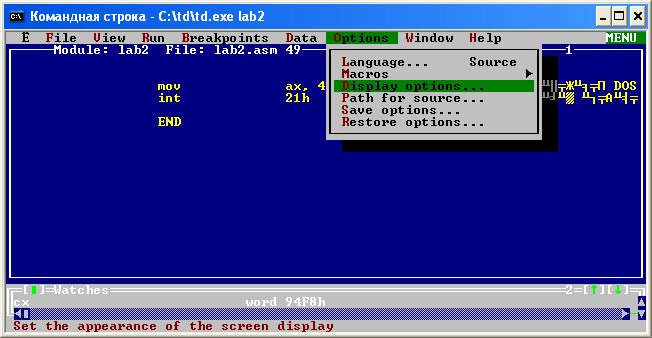
\includegraphics[width=.99\linewidth]
            {../_INCLUDES/task-4-13-2/1.png}
        \caption{1) \textbf{Display oprions}}
        \label{fig:task_4_13_2__1}
    \end{minipage}
    \begin {minipage}{0.32\textwidth}
        \centering
        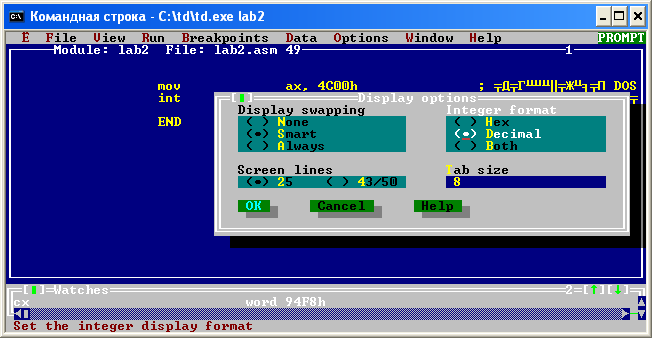
\includegraphics[width=.99\linewidth]
            {../_INCLUDES/task-4-13-2/2.png}
        \caption{2) Выбираем \textbf{Hex}}
        \label{fig:task_4_13_2__2}
    \end{minipage}
    \begin {minipage}{0.32\textwidth}
        \centering
        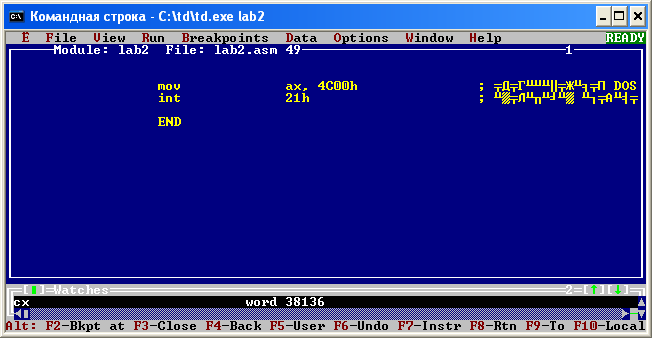
\includegraphics[width=.99\linewidth]
            {../_INCLUDES/task-4-13-2/3.png}
        \caption{3) Результат снизу}
        \label{fig:task_4_13_2__3}
    \end{minipage}
\end{figure}
